\section*{Tugas Modul} % Jika ada Tugas Modul
\begin{enumerate}
  \item Buatlah topologi jaringan percobaan 1, 2, dan 3!
  
  Topologi jaringan percobaan 1, 2, dan 3 dapat dilihat pada bagian \textbf{Topologi}.

  \item Perbedaan Point-to-Point, Point-to-Multipoint, dan Wireless Bridging!
      \begin{enumerate}
          \item Point-to-Point
          \begin{itemize}
              \item Koneksi langsung antara dua titik atau node dalam suatu jaringan.
              \item Terdapat dua titik akhir yang terhubung secara langsung tanpa perangkat tambahan diantaranya.
              \item Biasa digunakan untuk menghubungkan dua lokasi yang terpisah secara fisik.
              \item Cocok digunakan untuk aplikasi yang membutuhkan transmisi
          \end{itemize}
          \item Point-to-Multipoint: Topologi jaringan yang menghubungkan satu perangkat dengan beberapa perangkat lainnya.
          \begin{itemize}
              \item Koneksi dari suatu titik sender  yang mengirimkan data ke banyak titik receiver.
              \item Terdiri dari satu titik sender dan lebih dari satu titik receiver.
              \item Biasa digunakan pada public WiFi atau hotspot yang menyebarkan sinyal ke banyak pengguna.
              \item Mungkin digunakan untuk banyak perangkat untuk terhubung pada satu titik pusat.
          \end{itemize}
          \item Wireless Bridging: Topologi jaringan yang menghubungkan dua jaringan secara nirkabel.
          \begin{itemize}
              \item Koneksi wireless antara dua perangkat dengan konsep kabel LAN.
              \item Kedua segmen LAN berada dalam subnet yang sama dan terlihat seperti dua switch Ethernet yang dihubungkan oleh kabel.
              \item Biasa digunakan untuk menghubungkan dua lokasi fisik yang terpisah secara wireless, seperti gedung ke gedung atau bangunan ke bangunan.
          \end{itemize}
      \end{enumerate}
        
  \item Follow IG Lab MIOT ITS dan DM kami di @labmiotits dan @dm\_lab!
  
  Berikut ini adalah bukti kami telah mengikuti akun tersebut pada gambar \ref{fig:ig}:

  \begin{figure}[H]
    \centering
    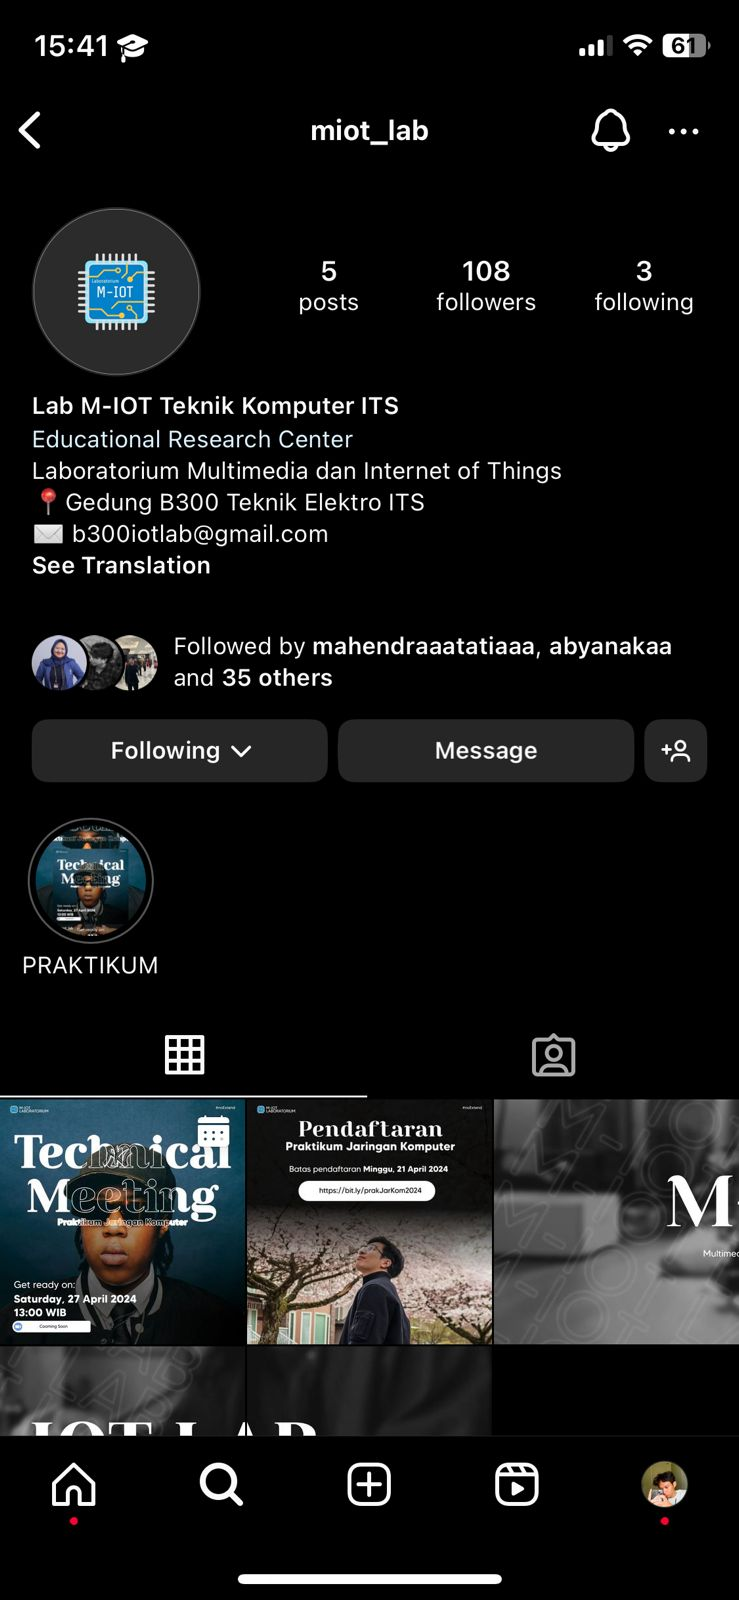
\includegraphics[width=0.4\textwidth]{img/ss_follow_b3.jpeg}
    \caption{Bukti Follow IG}
    \label{fig:ig}
  \end{figure}
        
\end{enumerate}